\chapter{Condensateurs}

\minisec{Objectif}

\begin{enumerate}
  \item L'étudiante saura ce qu'est un condensateur et comprendra le concept de
    capacité.
  \item L'étudiante sera en mesure de calculer la capacité de condensateurs dont
    la géométrie est simple.
  \item L'étudiante saura comment calculer l'énergie emmagasinée dans un
    condensateur.
  \item L'étudiante comprendra comment se comportent des condensateurs en série
    et en parallèle.
\end{enumerate}


\section{Condensateurs plans}

\marginnote{
  Tremblay \S 7.2

  Lafrance \S 5.2, 5.1
}

\begin{diapobox}
On considère deux grandes plaques parallèles connectées à une source de
tension.  Si on applique une différence de potentiel $\Delta V$ entre les deux
plaques, quelle charge sera emmagasinée sur chacune des plaques?

\begin{enumerate}
  \item Décrire le champ électrique entre les deux plaques.
  \item Déterminer le lien entre le champ électrique et la différence de
    potentiel.
  \item Montrer que la relation suivante est vraie
    $$Q = \frac{\epsilon_0 A}{d} \Delta V.$$
\end{enumerate}
\end{diapobox}


Un \textbf{condensateur} est constitué de deux \textbf{armatures} conductrices
portant des charges opposées séparées par un isolant. Dans un
\textbf{condensateur plan}, les armatures sont de très grandes plaques.

La \textbf{capacité} d'un condensateur décrit quelle charge peut être accumulée
sur l'armature positive pour chaque volt de différence de potentiel appliquée
entre les armatures. C'est une quantité qui ne dépend que de la géométrie du
condensateur et qui est reliée à la charge et à la différence de potentiel par
$$C = \frac{Q}{\Delta V}.$$

Dans le cas d'un condensateur plan
$$C = \frac{\epsilon_0 A}{d}.$$

Dans le système international, la capacité se mesure en farad (F). On note que
$$\SI{1}{\farad} = \SI{1}{\coulomb\per\volt}$$

\begin{center}
  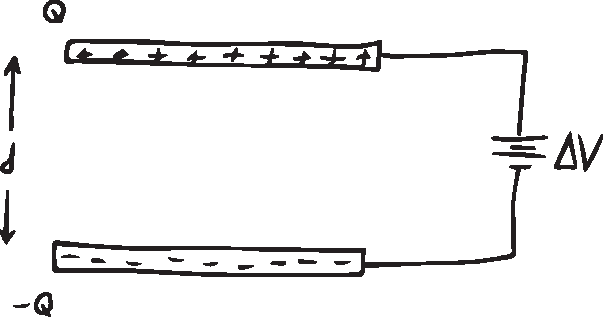
\includegraphics[scale=0.5]{05-condensateurs/figures/condensateur-plan.pdf}
\end{center}


\minisec{Propriétés de condensateurs plans}

\begin{diapobox}
Lequel des énoncés suivants est vrai.

\begin{enumerate}
  \item Si l'aire des plaques augmente, la capacité diminue.
  \item La charge accumulée sur un condensateur plan augmente
    proportionnellement à la différence de potentiel entre les plaques.
  \item Si on augmente la distance entre les plaques, l'énergie potentielle du
    condensateur diminue.
\end{enumerate}


Lequel des énoncés suivants est vrai.

\begin{enumerate}
  \item Plus la distance entre les plaques est grande, plus la différence de
    potentiel doit être élevée pour maintenir la même charge sur les plaques.
  \item Si la densité surfacique de charge augmente et que la différence de
    potentiel demeure la même, c'est parce que la distance entre les plaques a
    diminué.
  \item Pour un condensateur donné, plus la différence de potentiel entre les
    plaques augmente, plus la capacité diminue.
\end{enumerate}

\end{diapobox}



\subsection{Condensateurs et diélectriques}

\marginnote{
  Tremblay \S 7.7
}

\paragraph{Objectif}

\begin{enumerate}
  \item L'étudiante connaîtra la définition de la constante diélectrique.
  \item L'étudiante comprendra comment l'introduction d'un diélectrique
    influence la capacité d'un condensateur.
\end{enumerate}

\marginnote{10 minutes}

Demander aux étudiants de résumer comment l'introduction d'un condensateur
entre les armatures d'un condensateur chargé affecte le champ électrique, la
différence de potentiel et la capacité.

Les éléments suivants devraient se retrouver dans la description.

\begin{itemize}
  \item Diélectrique se polarise ce qui crée un champ électrique dans le
    diélectrique dans la direction opposé au champ électrique causé par les
    armatures.
  \item Par le principe de superposition, le champ électrique total a un module
    inférieur à celui des armatures seules.
  \item La différence de potentiel diminue du même facteur puisqu'elle est
    proportionnelle au champ électrique.
  \item La charge sur les armatures est la même, mais la différence de
    potentielle est plus faible, donc la capacité a augmenté (car $C = Q/\Delta
    V$).
\end{itemize}


\minisec{Constante diélectrique}

\marginnote{5 minutes}

Le champ électrique induit dans un diélectrique est en général proportionnel au
champ électrique externe et en sens opposé
$$\vE_\text{diel} = -\alpha \vE_\text{vide}$$
donc le champ électrique total est
$$\vE = \vE_\text{vide} + \vE_\text{diel} = (1 - \alpha) \vE_\text{vide}.$$
On définit la \textbf{constante diélectrique} comme
$$\kappa = \frac{1}{1 - \alpha}$$
c'est-à-dire que
$$\vE = \frac{1}{\kappa} \vE_\text{vide}.$$
Par conséquent, la différence de potentiel entre les plaques chute d'un facteur
$\kappa$ et la capacité devient
$$C = \frac{Q}{\Delta V / \kappa} = \kappa C_\text{vide}.$$


\minisec{Rigidité diélectrique}

Si le champ électrique externe appliqué sur un diélectrique est trop élevé, les
électrons seront arrachés aux atomes et un courant pourra traverser le
diélectrique. C'est ce qu'on appelle un \textbf{claquage}. Chaque matériau est
capable de supporter un champ électrique maximum qu'on appelle la
\textbf{rigidité diélectrique}. Le tableau ci-dessous donne la rigidité
diélectrique de quelques matériaux.

\begin{diapobox}
  \begin{center}
  \begin{tabular}{lS}
    \toprule
    Substance       &        {Rigidité diélectrique (\si{V/cm})}     \\
    \midrule
    Air             &  30000  \\
    Verre           &  100000 \\
    Polystyrène     &  197000 \\
    Papier ciré     &  500000 \\
    Diamant         &  20000000 \\
    \bottomrule
  \end{tabular}
  \end{center}
\end{diapobox}


\section{Énergie dans un condensateur chargé}

\marginnote{
  Tremblay \S 7.5

  Lafrance \S 5.3
}

On doit construire la configuration de charge, ie, calculer le travail
nécessaire pour amener chacune des charges à sa place sur le condensateur.

Considérons un condensateur avec une capacité $C$ dont les armatures sont
maintenues à une différence de potentiel $\Delta V$.

La différence de potentiel lorsque la charge est $q$ est
$$\Delta V = \frac{q}{C}$$
donc l'énergie requise pour amener une charge supplémentaire $dq$ est
\begin{align*}
  dU &= dq \Delta V \\
           &= \frac{q}{C} dq
\end{align*}
L'énergie totale est la somme des variations d'énergie pour chacune des petites
charges nécessaires pour faire passer la charge totale du condensateur de $0$ à
$Q$:
\begin{align*}
  \Delta U &= \int_0^Q \frac{q}{C} dq \\
           &= \left. \frac{q^2}{2C} \right|_0^Q \\
           &= \frac{Q^2}{2C}
\end{align*}



\minisec{Condensateur qui explose}

Si on applique une différence de potentiel trop élevée aux armatures d'un
condensateur, le champ électrique entre les armatures deviendra plus grand que
la rigidité diélectrique du matériel isolant et on assistera à une décharge.
Très souvent, un condensateur qui subit une décharge explosera tel qu'illustré
dans le vidéo suivant \url{https://youtu.be/XBoaBwMRbnk?t=30}.


\begin{diapobox}
Dans un des cas, on voit un condensateur de \SI{470}{\micro\farad} qui explose.
Supposons qu'il a explosé à une tension de \SI{200}{\volt}. Quelle est la
quantité d'énergie qui peut être relâchée durant cette explosion?
\end{diapobox}

\begin{reponsebox}
\begin{align*}
  U &= \frac{C\Delta V^2}{2}  \\
    &= \SI{9.40}{J}
\end{align*}

C'est environ l'énergie d'un bloc de \SI{1}{kg} qui tombe d'une hauteur de
\SI{1}{m} sur le bout de votre doigt...
\end{reponsebox}



\section{Circuits simples avec des condensateurs}

\marginnote{Tremblay \S 7.4}

\subsection*{Condensateurs en série}

\marginnote{15 minutes}

Si plusieurs condensateurs sont placés en série, est-ce que la capacité de
l'ensemble est plus grande, plus petite ou égale à la somme des capacités?

La charge accumulée sur chacun des condensateurs est la même parce les
armatures opposées doivent avoir des charges opposées, et chaque section du
circuit doit être électriquement neutre.

\begin{center}
  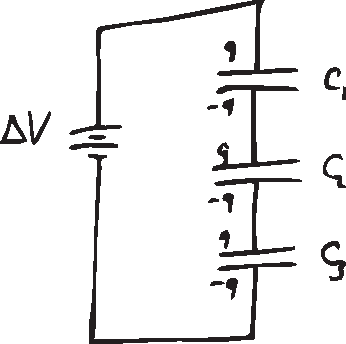
\includegraphics[scale=0.5]{05-condensateurs/figures/condensateur-serie.pdf}
\end{center}

De plus, la somme des différences de potentiel aux armatures de chacun des
condensateurs doit être la même que la différence de potentiel fournie par la
source. On a donc
\begin{align*}
  \Delta V &= \Delta V_1 + \Delta V_2 + \Delta V_3  \\
  \frac{q}{C_\mathrm{eq}} &= \frac{q}{C_1} + \frac{q}{C_2} + \frac{q}{C_3}  \\
  \frac{1}{C_\mathrm{eq}} &= \frac{1}{C_1} + \frac{1}{C_2} + \frac{1}{C_3}
\end{align*}



\subsection*{Condensateurs en parallèle}

\marginnote{15 minutes}

Dans le cas de condensateurs en parallèle, la charge accumulée sur chaque
condensateur n'est pas nécessairement la même, mais la ddp aux bornes de chaque
condensateur elle doit être identique. La charge qui sera accumulée sur un
condensateur équivalent aux trois condensateurs doit être la somme des charges
sur chaque condensateur.

\begin{center}
  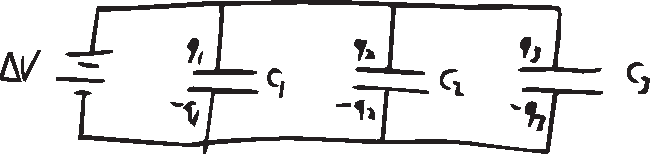
\includegraphics[scale=0.5]{05-condensateurs/figures/condensateur-parallele.pdf}
\end{center}

On a donc
\begin{align*}
  q &= q_1 + q_2 + q_3  \\
  C_\mathrm{eq} \Delta V &= C_1 \Delta V + C_2 \Delta V + C_3 \Delta V  \\
  C_\mathrm{eq} &= C_1 + C_2 + C_3
\end{align*}




\subsection*{Exemple}

On construit le circuit suivant avec une pile de \SI{9}{V}. Le condensateur 1 a
une capacité $C_1 = \SI{45}{\micro\farad}$ et ses armatures sont séparées par
du vide. Les condensateurs 2 et 3 sont construits exactement de la même façon que le
condensateur 1 sauf que tout l'espace entre leurs armatures est rempli par
du germanium et du papier, respectivement. La constante diélectrique du
germanium est 16 alors que celle du papier est 3.

\begin{center}
\begin{circuitikz}
  % French babel breaks everything... see https://latex.org/forum/viewtopic.php?t=11981
  \shorthandoff{:}\shorthandoff{!}
  \draw (0, 0) to[battery, l=$\SI{9}{\volt}$] (0, 3)
    to[C, l=$C_1$] (2, 3)
    to[C, l=$C_2$] (2, 0)
    to (0, 0);
  \draw (2, 3) to[short] (4, 3)
    to[C, l=$C_3$] (4, 0)
    to (2, 0);
\end{circuitikz}
\end{center}

\begin{enumerate}
  \item Déterminer la capacité équivalente à ces trois condensateurs.
  \item Déterminer la charge accumulée sur la plaque positive du condensateur 2.
  \item Déterminer l'énergie accumulée dans le condensateur 3.
\end{enumerate}


D'abord
\begin{align*}
  C_2 &= \kappa_\text{Ge} C_1 = 16C_1 = \SI{720}{\micro\farad} \\
  C_3 &= \kappa_\text{papier}C_1 = 3C_1 = \SI{135}{\micro\farad} \\
\end{align*}
$C_2$ et $C_3$ sont en parallèle donc
\begin{align*}
  C_{23} &= C_2 + C_3 \\
         &= \SI{855}{\micro\farad}
\end{align*}
$C_1$ est en série avec $C_{23}$ donc
\begin{align*}
  C_\text{eq} &= \frac{1}{\frac{1}{C_1} + \frac{1}{C_{23}}} \\
              &= \SI{42.8}{\micro\farad}
\end{align*}

La charge accumulée sur cette capacité équivalente serait la même que celle
accumulée sur $C_1$ et $C_{23}$. Donc
\begin{align*}
  Q_{23} &= C_\text{eq} \Delta V \\
         &= \SI{384.75}{\micro\coulomb}
\end{align*}
La différence de potentiel aux bornes de $C_2$ (et $C_3$) est donc
\begin{align*}
  \Delta V_{2} &= \frac{Q_{23}}{C_{23}} \\
               &= \SI{0.45}{\volt}
\end{align*}
d'où on peut déduire la charge accumulée sur $C_2$
\begin{align*}
  Q_2 &= C_2 \Delta V_2 \\
      &= \SI{324}{\micro\coulomb}
\end{align*}

L'énergie emmagasinée dans $C_3$ est obtenue par
\begin{align*}
  U_3 &= \frac{Q_3^2}{2C_3} = \frac{C_3 \Delta V_3^2}{2}  \\
      &= \SI{13.67}{\micro\joule}
\end{align*}



